\documentclass[twocolumn]{article}
\usepackage[margin=0.75cm]{geometry}
\usepackage{hyperref}
\hypersetup{
    colorlinks,
    citecolor=blue,
    filecolor=blue,
    linkcolor=blue,
    urlcolor=blue
}

\usepackage{graphicx, caption, multirow, mathtools, amsfonts, booktabs, siunitx, bbold}
\setlength{\columnseprule}{.75pt}
\def\columnseprulecolor{\color{black}}
\newcommand{\overbar}[1]{\mkern 1.5mu\overline{\mkern-1.5mu#1\mkern-1.5mu}\mkern 1.5mu}
\DeclareMathOperator*{\argmax}{argmax}
\DeclareMathOperator*{\argmin}{argmin}

\usepackage{tikz}
\usetikzlibrary{positioning, arrows, fit}

\setlength{\parindent}{0pt}
\setlength{\parskip}{6pt}

\everymath{\displaystyle}

% for box
\usepackage{tcolorbox}
\tcbuselibrary{theorems}
\newtcbtheorem[]{mydef}{}{colback=gray!5, colframe=black!75, fonttitle=\bfseries}{th}

\title{
	\vspace{-2em}
	\normalsize \textbf{Reinforcement Learning Formula Sheet} \\
	\small Eddie Guo \\
	\dotfill
	\vspace{-5em}
}
\date{}

\begin{document}
\maketitle

\small

\textbf{Multi-Armed Bandit Problem}

Expected reward of action $a$: $q_*(a) \equiv \mathbb E [R_t \mid A_t = a]$

Estimate of $q_*(a)$ at time $t$: $Q_t(a) \equiv \frac{\sum_{i=1}^{t-1} R_i \cdot \mathbb 1_{A_i = a}}{\sum_{i=1}^{t-1} \mathbb 1_{A_i = a}}$

$\quad$Optimization: $Q_{n+1} = Q_n + \frac{1}{n} (R_n - Q_n)$

$\quad \lim_{t \to \infty} Q_t(a) = q_*(a)$ by LLN

\textit{Greedy action selection:} $A_t = \argmax_a Q_t(a)$

\textit{$\epsilon$-greedy selection:} greedy most of time but selects random action w/ small probability $\epsilon$

\textit{Nonstationary problems: constant step-size parameter}

$\quad Q_{n+1} \equiv Q_n + \alpha (R_n - Q_n), \quad \alpha \in [0, 1)$

$\quad Q_{n+1} = (1-\alpha)^n Q_1 + \sum_{i=1}^n \alpha (1-\alpha)^{n-i} R_i$

$\quad$Notice exponentially decaying past rewards.

\begin{mydef}{A simple bandit algorithm}{}
    Initialize, for $a$ = 1 to $k$: \\
        \hspace*{2em} $Q(a) \leftarrow 0$ \\
        \hspace*{2em} $N(a) \leftarrow 0$ \\
    Loop: \\
        \hspace*{2em} $A \leftarrow \begin{cases} \argmax_a Q(a), & \text{with probability 1 - $\epsilon$}\\ \text{random action}, & \text{with probability $\epsilon$} \end{cases}$ \\
        \hspace*{2em} $R \leftarrow bandit(A)$ \\
        \hspace*{2em} $N(A) \leftarrow N(A) + 1$ \\
        \hspace*{2em} $Q(A) \leftarrow Q(A) + \frac{1}{N(A)} [R-Q(A)]$
\end{mydef}

\vspace{-.5em}
\dotfill

\textit{Upper Confidence Bound (UCB) Action Selection}

``Optimism in the face of uncertainty''

Same as greedy except initialize $Q_t(a)$ to a high value, select value that optimizes an action $A_t$, and updates the upper bound to $Q_t(a)$.

$\quad A_t \equiv \argmax \left[ Q_t(a) + c \sqrt{\frac{\ln t}{N_t(a)}} \right]$

\dotfill

\textbf{Finite Markov Decision Processes}

State: $S_t \in \mathcal{S}$, \hfill Action: $A_t \in \mathcal{A}(s)$, \hfill Reward: $R_{t+1} \in \mathcal{R} \subset \mathbb{R}$

Transition dynamics fn (joint PMF):

$\quad$Joint prob of next state $s'$ and reward $r$ given state $s$ and action $a$.

$\quad p(s', r \mid s, a) \equiv \Pr \{ S_t = s', R_t = r \mid S_{t-1} = s, A_{t-1} = a \}$

$\quad p: \mathcal S \times \mathcal R \times \mathcal S \times \mathcal A \to [0, 1]$

$\quad \sum_{s' \in \mathcal S} \sum_{r \in \mathcal R} p(s', r \mid s, a) = 1, \quad \forall s \in \mathcal S, \forall a \in \mathcal A(s)$

\vspace{-1em}\begin{figure}[h!]
    \centering
    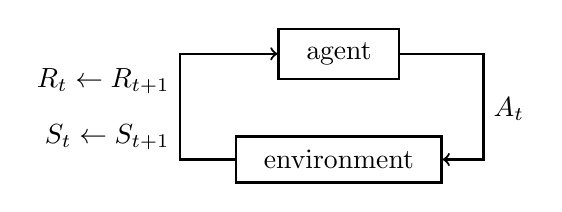
\begin{tikzpicture}
        \tikzset{
            rect/.style={draw, thick, rectangle, align=center, inner xsep=1em, inner ysep=.5em}
        }
        
        \node (origin) at (0, 0) {};
        \node (agent) [rect, right=2em of origin] {agent};
        \node (envir) [rect, below=2em of agent] {environment};
        % arrows
        \draw [thick, ->] (agent.east) -| node [right, yshift=-2em] {$A_t$} ++(3em, 0) |- (envir.east);
        \draw [thick, ->] (envir.west) -| ++(-2em, 0) |- node [left, yshift=-1em] {$R_t \leftarrow R_{t+1}$} node [left, yshift=-3em] {$S_t \leftarrow S_{t+1}$} (agent.west);
    \end{tikzpicture}
\end{figure}

\textit{State-Transition Probabilities (Alternative Forms)}

$p(s', r \mid s,a) \equiv \Pr \{ S_t = s', R_t = r \mid S_{t-1} = s, A_{t-1} = a \}$

$p(s' \mid s, a) = \Pr \{ S_t = s' \mid S_{t-1} = s, A_{t-1} = a \} = \sum_{r \in \mathcal R} p(s', r \mid s, a)$

$r(s, a) \equiv \mathbb E [R_t \mid S_{t-1} = s, A_{t-1} = a] = \sum_{r \in \mathcal R} r \sum_{s' \in \mathcal S} p(s', r \mid s, a)$

$r(s, a, s') \equiv \mathbb E [R_t \mid S_{t-1} = s, A_{t-1} = a, S_t = s'] = \sum_{r \in \mathcal R} r \frac{p(s', r \mid s, a)}{p(s' \mid s, a)}$

\dotfill

Markov property: future states of Markov process depend only on present state and not on past events.

Agent-envir interactions: episode $\to$ terminal state $\to$ reset

Goal of agent: maximize expected return, $G_t$

Episodic tasks: $G_t \equiv R_{t+1} + R_{t+2} + \cdots + R_T$

\vspace{-.5em}
\dotfill

\textit{Continuing Tasks (no terminal state)}

$G_t \equiv R_{t+1} + \gamma R_{t+2} + \gamma^2 R_{t+3} + \cdots + \gamma^{k-1} R_{t+k} + \cdots = \sum_{k=0}^\infty \gamma^k R_{t+k+1}$

$G_t = R_{t+1} + \gamma G_{t+1}$, \hfill $\sum_{k=0}^\infty \gamma^k = \frac{1}{1-\gamma},$ \hfill $\gamma \in [0, 1)$ is discount rate

$G_t \equiv \sum_{k=t+1}^T \gamma^{k-t-1} R_k$ \hfill $T = \infty$ or $\gamma = 1$ (but not both)

Notice that future rewards are discounted more.

$\quad \gamma = 0$: agent only cares about immediate reward (greedy).

$\quad \gamma \to 1$: future rewards contribute more.

\vspace{-.5em}
\dotfill

\textbf{Policies}

Law of total expectation: $\mathbb E[X] = \mathbb E[\mathbb E[X \mid Y]]$

$\quad$Partition formula: $\mathbb E[X] = \sum_i \mathbb E[X \mid A_i] P(A_i)$

Policy: mapping from states to probs of selecting each possible action.

$\quad \pi(a|s)= p(a \mid s) = \Pr \{ A_t = a \mid S_t = s \}$

Expectation of $R_{t+1}$ in terms of $\pi$ and $p$:

$\quad \mathbb E[R_{t+1} \mid S_t = s] = \sum_a \pi(a \mid S_t) \sum_{s', r} p(s', r \mid s, a) r$

\dotfill

\textbf{Value Functions}

Value fns give expected return $G_t$ when starting in state $s$ and following policy $\pi$ thereafter.

\textit{State-value fn:} $v_\pi(s) \equiv \mathbb E_\pi [G_t \mid S_t = s]$ \hfill $G_t = \sum_{k=0}^\infty \gamma^k R_{t+k+1}$

$\quad$Value of terminal state is always 0.

\textit{Action-value fn:} $q_\pi(s, a) \equiv \mathbb E_\pi [G_t \mid S_t = s, A_t = a]$

$\quad v_\pi$ in terms of $q_\pi$ and $\pi$: $v_\pi (s) = \sum_a \pi(a \mid S_t) q_\pi(s, a)$

$\quad q_\pi$ in terms of $v_\pi$ and $p$: $q_\pi(s, a) = \sum_{r, s'} p(s', r \mid s, a) [r + \gamma v_\pi(s')]$


\cleardoublepage


\textbf{Bellman Equations}

$v_\pi(s) = \sum_a \pi(a \mid s) \sum_{s', r} p(s', r \mid s, a) [r + \gamma v_\pi(s')]$

$q_\pi(s,a) = \sum_{s', r} p(s',r \mid s,a) \left[ r + \gamma \sum_{a'} \pi(a' \mid s') q(s', a') \right]$

\textit{Optimal value fns:} $\pi_1 \geq \pi_2 \iff v_{\pi_1}(s) \geq v_{\pi_2}(s), \quad \forall s \in \mathcal S$

$\quad v_*(s) = \max_\pi v_{\pi}(s) = \max_a \sum_{s', r} p(s', r \mid s, a) [r + \gamma v_*(s')], \quad \forall s \in \mathcal S$

$\quad q_*(s, a) = \max_{\pi} q_\pi(s,a) = \sum_{s', r} p(s', r \mid s, a) [ r + \gamma \max_{a'} q_*(s', a')]$

$\quad \quad \forall s \in \mathcal S, \forall a \in \mathcal A$

\vspace{-.5em}
\dotfill

\textbf{Policy Evaluation}

$\pi_* = \argmax_a \sum_{s', r} p(s',r \mid s, a)[r + \gamma v_*(s')]$

\begin{mydef}{Iterative Policy Evaluation}{}
    Input $\pi$, the policy to be evaluated \\
    $\vec V \leftarrow \vec 0, \vec V' \leftarrow \vec 0$ \\
    loop: \\
        \hspace*{2em} $\Delta \leftarrow 0$ \\
        \hspace*{2em} loop for each $s \in \mathcal S$: \\
            \hspace*{4em}$V'(s) \leftarrow \sum_a \pi(a \mid s) \sum_{s', r} p(s', r \mid s, a) [r + \gamma V(s')]$ \\
            \hspace*{4em}$\Delta \leftarrow \max(\Delta, |V'(s) - V(s)|)$ \\
        \hspace*{2em}$V \leftarrow V'$ \\
    until $\Delta < \theta$ (small positive number) \\
    return $V \approx v_\pi$
\end{mydef}

\textit{Policy improvement thm:} $q_\pi(s, \pi'(s)) \geq v_\pi(s), \quad \forall s \in \mathcal S$

$\pi'(s) \equiv \argmax_a q_\pi(s,a) = \argmax_a \sum_{s', r} p(s',r \mid s,a) [r + \gamma v_\pi(s')]$

\begin{mydef}{Policy Iteration}{}
    1. Initialization \\
    $V(s) \in \mathbb R$ and $\pi(s) \in \mathcal A(s)$ arbitrarily $\forall s \in \mathcal S$ \\
    
    2. Policy Evaluation \\
    Loop: \\
        \hspace*{2em}$\Delta \leftarrow 0$ \\
        \hspace*{2em}Loop for each $s \in \mathcal S:$ \\
            \hspace*{4em}$v \leftarrow V(s)$ \\
            \hspace*{4em}$V(s) \leftarrow \sum_{s', r} p(s', r \mid s, \pi(s)) [r + \gamma V(s')]$ \\
            \hspace*{4em}$\Delta \leftarrow \max(\Delta, |v - V(s)|)$ \\
    
    3. Policy Improvement \\
    \textit{policy-stable} $\leftarrow$ true \\
    For each $s \in \mathcal S$: \\
        \hspace*{2em}\textit{old-action} $\leftarrow \pi(s)$ \\
        \hspace*{2em}$\pi(s) \leftarrow \argmax_a \sum_{s', r} p(s', r \mid s,a)[r + \gamma V(s')]$ \\
        \hspace*{2em}If \textit{old-action} $\neq \pi(s)$, then \textit{policy-stable} $\leftarrow$ false \\
    If \textit{policy-stable}, then stop and return $V \approx v_*$ and $\pi \approx \pi_*$; else go to 2.
\end{mydef}

\newpage

\textbf{Monte Carlo Methods}

\vspace{-.5em}\begin{itemize}
    \item Reqs only sample sequences of states, actions, rewards from interactions w/ envir. Works in RL by averaging sample returns.
    \item MC only for episodic tasks b/c only upon completion of episode are value estimates and policies changed.
\end{itemize} \vspace{-.5em}

\begin{mydef}{First-visit MC prediction for estimating $V \approx v_\pi$}{}
    Input: policy $\pi$ to be evaluated \\

    Initialize: \\
        \hspace*{2em}$V(s) \in \mathbb R$, arbitrarily $\forall s \in \mathcal S$ \\
        \hspace*{2em}$Returns(s) \leftarrow$ empty list $\forall s \in \mathcal S$ \\

    Loop (for each episode): \\
        \hspace*{2em}Generate episode following $\pi$ \\
        \hspace*{2em}$G \leftarrow 0$ \\
        \hspace*{2em}Loop for each step of episode, $t = T-1, T-2, \dots, 0$: \\
            \hspace*{4em}$G \leftarrow \gamma G + R_{t+1}$ \\
            \hspace*{4em}Unless $S_t$ appears in $S_0, S_1, \dots, S_{t-1}$: \\
                \hspace*{6em}Append $G$ to $Returns(S_t)$ \\
                \hspace*{6em}$V(S_t) \leftarrow \text{average}(Returns(S_t))$
\end{mydef}

\dotfill

\textit{MC Estimation of Action Values}

$\pi(s) \equiv \argmax_a q(s,a)$, \hfill $q_{\pi_k}(s, \pi_{k+1}(s)) \geq q_{\pi_k}(s, \pi_k(s)) \geq v_{\pi_k}(s)$

\begin{mydef}{First-visit MC prediction for estimating $V \approx v_\pi$}{}
    Input: policy $\pi$ to be evaluated \\

    Initialize: \\
        \hspace*{2em}$\pi(s) \in \mathcal A(s)$, arbitrarily $\forall s \in \mathcal S$ \\
        \hspace*{2em}$Q(s, a) \in \mathbb R$, arbitrarily $\forall s \in \mathcal S, \forall a \in \mathcal A$ \\
        \hspace*{2em}$Returns(s) \leftarrow$ empty list $\forall s \in \mathcal S, \forall a \in \mathcal A$ \\

    Loop (for each episode): \\
        \hspace*{2em}Choose $S_0 \in \mathcal S, A_0 \in \mathcal A(S_0)$ randomly st all pairs have probabilities greater than $0$ \\
        \hspace*{2em}Generate episode from $S_0, A_0$ following $\pi$ \\
        \hspace*{2em}$G \leftarrow 0$ \\
        \hspace*{2em}Loop for each step of episode, $t = T-1, T-2, \dots, 0$: \\
            \hspace*{4em}$G \leftarrow \gamma G + R_{t+1}$ \\
            \hspace*{4em}Unless $S_t$ appears in $S_0, A_0, \dots, S_{t-1}, A_{t-1}$: \\
                \hspace*{6em}Append $G$ to $Returns(S_t)$ \\
                \hspace*{6em}$Q(S_t, A_t) \leftarrow \text{average}(Returns(S_t, A_t))$ \\
                \hspace*{6em}$\pi(S_t) \leftarrow \argmax_a Q(S_t, a)$
\end{mydef}

Note the last three lines can be made more efficient:

$Q(S_t, A_t) \leftarrow Q(S_t, A_t) + \frac{1}{n} (G - Q(S_t, A_t))$

$\pi(S_t) \leftarrow \argmax_a Q(S_t, a))$

\vspace{-.5em}
\dotfill

\textit{MC Control w/o Exploring Starts}

On-policy: tries to evaluate or improve policy used to make decisions.

Off-policy: same as on-policy but policy is different from that used to generate data: target policy + behaviour policy.

$\epsilon$-soft policy: all nongreedy actions given minimal probability of selection $\epsilon / | \mathcal A(s)|$ whereas greedy action given probability $1 - \epsilon + \epsilon/| \mathcal A(s)|$.


\cleardoublepage


\begin{mydef}{On-policy first-visit MC control (for $\epsilon$-soft policies, $\pi \approx \pi_*$)}{}
    Algorithm parameter: small $\epsilon > 0$ \\

    Initialize: \\
        \hspace*{2em}$\pi \leftarrow$ arbitrary $\epsilon$-soft policy \\
        \hspace*{2em}$Q(s, a) \in \mathbb R$, arbitrarily $\forall s \in \mathcal S, \forall a \in \mathcal A$ \\
        \hspace*{2em}$Returns(s) \leftarrow$ empty list $\forall s \in \mathcal S, \forall a \in \mathcal A$ \\

    Loop (for each episode): \\
        \hspace*{2em}Generate episode from $S_0, A_0$ following $\pi$ \\
        \hspace*{2em}$G \leftarrow 0$ \\
        \hspace*{2em}Loop for each step of episode, $t = T-1, T-2, \dots, 0$: \\
            \hspace*{4em}$G \leftarrow \gamma G + R_{t+1}$ \\
            \hspace*{4em}Unless pair $S_t, A_t$ appears in $S_0, A_0, \dots, S_{t-1}, A_{t-1}$: \\
                \hspace*{6em}Append $G$ to $Returns(S_t)$ \\
                \hspace*{6em}$Q(S_t, A_t) \leftarrow \text{average}(Returns(S_t, A_t))$ \\
                \hspace*{6em}$A^* \leftarrow \argmax_a Q(S_t, a)$ \\
                \hspace*{6em}$\forall a \in \mathcal A(S_t)$: \\
                    \hspace*{8em}$\pi(a \mid S_t) \leftarrow \begin{cases}
                        1 - \epsilon + \epsilon / |A(S_t)| & \text{if } a = A^* \\
                        \epsilon / |A(S_t)| & \text{if } a \neq A^*
                    \end{cases}$
\end{mydef}

\dotfill

\textit{Off-Policy Prediction via Importance Sampling}

$\Pr \{ A_t, S_{t+1}, A_{t+1}, \dots, S_T \mid S_t, A_{t:T-1} \sim \pi \} = \prod_{k=t}^{T-1} \pi(A_k \mid S_k) p(S_{k+1} \mid S_k, A_k)$

$\mathbb E [G_t \mid S_t = s] = v_b(s)$ \hfill $\mathbb E [\rho_{t:T-1} G_t \mid S_t = s] = v_\pi(s)$

$\quad \rho_{t:T-1} = \prod_{k=t}^{T-1} \frac{\pi(A_k \mid S_k)}{b(A_k \mid S_k)}$

Ordinary importance sampling: $V(s) \equiv \frac{\sum_{t \in \mathcal T(s)} \rho G_t}{|\mathcal T(s)|}$

Weighted importance sampling: $V(s) \equiv \frac{\sum_{t \in \mathcal T(s)} \rho G_t}{\sum_{t \in \mathcal T(s)} \rho}$

Ordinary unbiased w/ high variance; weighted is biased w/ lower variance (preferred method).

\vspace{-.5em}
\dotfill

\textit{Incremental Implementation}

Suppose we have seq of returns $G_1, G_2, \dots, G_{n-1}$ all starting from same state with random weight $W_i$. We wish to estimate
\begin{equation*}
    V_n \equiv \frac{\sum_{k=1}^{n-1}} W_k G_k{\sum_{k=1}^{n-1} W_k}, \quad n \geq 2
\end{equation*}

We can use the following equation:
\begin{equation*}
    V_{n+1} \equiv V_n + \frac{W_n}{C_n} (G_n - V_n), \quad n \geq 1
\end{equation*}
where $C_{n+1} \equiv C_n + W_{n+1}$ and $C_0 = 0$ ($C_n$ is sum of weights).

\newpage

\begin{mydef}{Off-policy MC prediction (policy evaluation) $Q \approx Q_\pi$)}{}
    Input: an arbitrary target policy $\pi$ \\
    
    Initialize, $\forall s \in \mathcal S, a \in \mathcal A(s)$: \\
        \hspace*{2em}$Q(s,a) \in \mathbb R$ (arbitrarily) \\
        \hspace*{2em}$C(s,a) \leftarrow 0$ \\
    
        Loop (for each episode): \\
            \hspace*{2em}$b\leftarrow$ any policy w/ coverage of $\pi$ \\
            \hspace*{2em}Generate an episode following $b: S_0, A_0, R_1, \dots$ \\
            \hspace*{2em}$G \leftarrow 0$ \\
            \hspace*{2em}$W \leftarrow 1$ \\
            \hspace*{2em}Loop for each step of episode, $t = T-1, T-2, \dots, 0$ while $W \neq 0$: \\
                \hspace*{4em}$G \leftarrow \gamma G + R_{t+1}$ \\
                \hspace*{4em}$C(S_t, A_t) \leftarrow C(S_t, A_t) + W$ \\
                \hspace*{4em}$Q(S_t, A_t) \leftarrow Q(S_t, A_t) + \frac{W}{C(S_t, A_t)} [G - Q(S_t, A_t)]$ \\
                \hspace*{4em}$W \leftarrow W \frac{\pi(A_t \mid S_t)}{b(A_t \mid S_t)}$
\end{mydef}

\begin{mydef}{Off-policy MC control $\pi \approx \pi_*$}{}
    Initialize, $\forall s \in \mathcal S, a \in \mathcal A(s)$: \\
        \hspace*{2em}$Q(s,a) \in \mathbb R$ (arbitrarily) \\
        \hspace*{2em}$C(s,a) \leftarrow 0$ \\
        \hspace*{2em}$\pi(s) \leftarrow \argmax_a Q(s, a)$
    
        Loop (for each episode): \\
            \hspace*{2em}$b\leftarrow$ any policy w/ coverage of $\pi$ \\
            \hspace*{2em}Generate an episode following $b: S_0, A_0, R_1, \dots$ \\
            \hspace*{2em}$G \leftarrow 0$ \\
            \hspace*{2em}$W \leftarrow 1$ \\
            \hspace*{2em}Loop for each step of episode, $t = T-1, T-2, \dots, 0$: \\
                \hspace*{4em}$G \leftarrow \gamma G + R_{t+1}$ \\
                \hspace*{4em}$C(S_t, A_t) \leftarrow C(S_t, A_t) + W$ \\
                \hspace*{4em}$Q(S_t, A_t) \leftarrow Q(S_t, A_t) + \frac{W}{C(S_t, A_t)} [G - Q(S_t, A_t)]$ \\
                \hspace*{4em}$\pi(S_t) \leftarrow \argmax_a Q(S_t, a)$ \\
                \hspace*{4em}If $A_t \neq \pi(S_t)$ then exit inner Loop \\
                \hspace*{4em}$W \leftarrow W \frac{1}{b(A_t \mid S_t)}$
\end{mydef}

\dotfill

\textbf{Temporal-Difference Learning}

TD(0) update: $V(S_t) \leftarrow V(S_t) + \alpha [R_{t+1} + \gamma V(S_{t+1}) - V(S_t)]$

TD error: $\delta_t \equiv R_{t+1} + \gamma V(S_{t+1}) - V(S_t)$

\begin{mydef}{Tabular TD(0) for estimating $v_\pi$}{}
    Input: policy $\pi$ to be evaluated \\
    Algorithm parameter: step size $\alpha \in (0, 1]$ \\
    Initialize $V(s)$, $\forall s \in \mathcal S$ arbitrarily except $V(\text{terminal}) = 0$ \\
    
        Loop (for each episode): \\
            \hspace*{2em}Initialize $S$ \\
            \hspace*{2em}Loop for each step of episode: \\
                \hspace*{4em}$A \leftarrow$ action given by $\pi$ for $S$ \\
                \hspace*{4em}Take action $A$, observe $R, S'$ \\
                \hspace*{4em}$V(s) \leftarrow V(s) + \alpha [R + \gamma V(s') - V(s)]$ \\
                \hspace*{4em}$S \leftarrow S'$ \\
            \hspace*{2em}until $S$ is terminal
\end{mydef}


\cleardoublepage

MC error: $G_t - V(S_t) = \sum_{k=t}^{T-1} \gamma^{k-t} S_t$

\dotfill

\textbf{Sarsa: On-Policy TD Control}

$Q(S_t, A_t) \leftarrow Q(S_t, A_t) + \alpha [R_{t+1} + \gamma Q(S_{t+1}, A_{t+1}) - Q(S_t, A_t)]$

\begin{mydef}{Sarsa (on-policy TD control) for estimating $Q \approx q_*$}{}
    Algorithm parameter: step size $\alpha \in (0, 1]$, small $\epsilon > 0$ \\
    Initialize $Q(s,a)$, $\forall s \in \mathcal S, a \in \mathcal A(s)$ arbitrarily except $Q(\text{terminal}, \cdot) = 0$ \\
    
        Loop (for each episode): \\
            \hspace*{2em}Initialize $S$ \\
            \hspace*{2em}Choose $A$ from $S$ using policy derived from $Q$: \\
            \hspace*{2em}Loop for each step of episode: \\
                \hspace*{4em}Take action $A$, observe $R, S'$ \\
                \hspace*{4em}Choose $A'$ from $S'$ using policy derived from $Q$ \\
                \hspace*{4em}$Q(S,A) \leftarrow Q(S,A) + \alpha[R + \gamma Q(S', A') - Q(S, A)]$ \\
                \hspace*{4em}$S \leftarrow S'; A \leftarrow A'$ \\
            \hspace*{2em}until $S$ is terminal
\end{mydef}

\dotfill

\textbf{Q-Learning: Off-Policy TD Control}

$Q(S_t, A_t) \leftarrow Q(S_t, A_t) + \alpha [R_{t+1} + \gamma \max_a Q(S_{t+1}, a) - Q(S_t, A_t)]$

\begin{mydef}{Q-learning (off-policy TD control) for estimating $\pi \approx \pi_*$}{}
    Algorithm parameter: step size $\alpha \in (0, 1]$, small $\epsilon > 0$ \\
    Initialize $Q(s,a)$, $\forall s \in \mathcal S, a \in \mathcal A(s)$ arbitrarily except $Q(\text{terminal}, \cdot) = 0$ \\
    
        Loop (for each episode): \\
            \hspace*{2em}Initialize $S$ \\
            \hspace*{2em}Choose $A$ from $S$ using policy derived from $Q$: \\
            \hspace*{2em}Loop for each step of episode: \\
                \hspace*{4em}Choose $A$ from $S$ using policy derived from $Q$ \\
                \hspace*{4em}Take action $A$, observe $R, S'$ \\
                \hspace*{4em}$Q(S,A) \leftarrow Q(S,A) + \alpha[R + \max_a \gamma Q(S', a) - Q(S, A)]$ \\
                \hspace*{4em}$S \leftarrow S'$ \\
            \hspace*{2em}until $S$ is terminal
\end{mydef}

Double $Q$-learning addresses maximization bias problem. Instead of single $Q(S,A)$ update, with 0.5 probability, choose one of:
\begin{equation*}
    \begin{cases}
        Q_1(S,A) + \alpha \left( R + \gamma Q_2(S', \argmax_a Q_1(S', a)) - Q_1(S, A) \right) \\
        Q_2(S,A) + \alpha \left( R + \gamma Q_1(S', \argmax_a Q_2(S', a)) - Q_2(S, A) \right)
    \end{cases}
\end{equation*}
Can adapt this for Sarsa and expected Sarsa updates.

\vspace{-.5em}
\dotfill


\textbf{Expected Sarsa}

$Q(S_t, A_t)$

$\quad \leftarrow Q(S_t, A_t) + \alpha [R_{t+1} + \gamma \mathbb E_\pi [Q(S_{t+1}, A_{t+1}) \mid S_{t+1}] - Q(S_t, A_t)]$

$\quad\leftarrow Q(S_t, A_t) + \alpha[R_{t+1} + \gamma \sum_a \pi(a \mid S_{t+1}) Q(S_{t+1}, a) - Q(S_t, A_t)]$

Eliminates variance due to random selection of $A_{t+1}$ from Sarsa.


\newpage


\textbf{Models and Planning}

model $\xrightarrow{\text{planning}}$ policy

\begin{mydef}{Random-sample one-step tabular Q-planning}{}
    Loop:
    \begin{enumerate}
        \item Select a state, $S \in \mathcal S$ and action, $A \in \mathcal A(S)$, at random
        \item Send $S, A$ to a sample model and obtain sample next reward $R$ and sample next state $S'$
        \item Apply one-step tabular Q-learning to $S, A, R, S'$: \\
        $Q(S, A) \leftarrow Q(S, A) + \alpha [R + \gamma \max_a Q(S', a) - Q(S, A)]$
    \end{enumerate}
\end{mydef}

\dotfill

\textbf{Dyna-Q}

\begin{mydef}{Tabular Dyna-Q}{}
    Initialize $Q(s,a)$ and $Model(s,a),\ \forall s \in \mathcal S, a \in \mathcal A(s)$ \\
    Loop:
    \begin{enumerate}
        \item $S \leftarrow$ current (nonterminal) state
        \item $A \leftarrow \epsilon$-greedy($S,Q$)
        \item Take action $A$; observe resultant reward $R$ and state $S'$
        \item $Q(S,A) \leftarrow Q(S,A) + \alpha[R + \gamma \max_a Q(S',a) - Q(S, A)]$
        \item $Model(S,A) \leftarrow R, S'$ (assuming deterministic envir)
        \item Loop repeat $n$ times:
        \subitem$S \leftarrow$ random previously observed state
        \subitem$A \leftarrow$ random action previously taken in $S$
        \subitem$R,S' \leftarrow Model(S,A)$
        \subitem$Q(S,A) \leftarrow Q(S,A) + \alpha [R + \gamma \max_a Q(S', a) - Q(S,A)]$
    \end{enumerate}
\end{mydef}

Dyna-Q+ has reward of $r + \kappa \sqrt{\tau}$, where $\kappa$ is a constant and $\tau$ is the number of time steps since a given transition.

\vspace{-.5em}
\dotfill

\textbf{n-Step Bootstrapping}

\begin{mydef}{$n$-step TD for estimating $V \approx v_\pi$}{}
    Input: policy $\pi$ to be evaluated \\
    Algorithm parameters: step size $\alpha \in (0, 1]$, positive integer $n$ \\
    Initialize $V(s)$, arbitrarily $\forall s \in \mathcal S$ \\
    All store and access operations (for $S_t$ and $R_t$) can take their index mod ($n+1$) \\
    
    Loop (for each episode): \\
        \hspace*{2em}Initialize and store $S_0 \neq$ terminal \\
        \hspace*{2em}$T \leftarrow \infty$ \\
        \hspace*{2em}Loop for $t=0,1,2,\dots$: \\
            \hspace*{4em}If $t < T$, then: \\
                \hspace*{6em}Take an action according to $\pi(\cdot \mid S_t)$ \\
                \hspace*{6em}Observe and store $R_{t+1}, S_{t+1}$ \\
                \hspace*{6em}If $S_{t+1}$ terminal, then $T \leftarrow t+1$ \\
            \hspace*{4em}$\tau \leftarrow t-n+1$ \\
            \hspace*{4em}If $\tau \geq 0$: \\
                \hspace*{6em}$G \leftarrow \sum_{i=\tau+1}^{\min (\tau+n, T)} \gamma^{i-\tau-1} R_i$ \\
                \hspace*{6em}If $\tau + n < T$, then: $G \leftarrow G + \gamma^n V(S_{\tau+n})$ \\
                \hspace*{6em}$V(S_\tau) \leftarrow V(S_\tau) + \alpha [G-V(S_\tau)]$ \\
        \hspace*{2em}Until $\tau=T-1$
\end{mydef}


\cleardoublepage


\textbf{Prediction Objective}

$\overline{VE} \equiv \sum_{s \in \mathcal S} \mu(s)[v_\pi(s) - \hat v(s, \mathbf w)]^2$ \hfill $\mu(s) \geq 0, \quad \sum_s \mu(s) = 1$

Goal: $\overline{VE}(\mathbf w^*) \leq \overline{VE}(\mathbf w),\ \forall \mathbf w$

$\mu(s)$ is often the fraction of time spent in state $s$

\vspace{-.5em}
\dotfill

\textbf{Stochastic-Gradient and Semi-Gradient Methods}

$\mathbf w_{t+1} \equiv \mathbf w_t - \frac{1}{2}\alpha \nabla[v_\pi(S_t) - \hat v(S_t, \mathbf w_t)]^2$

$\hspace{2.5em} = \mathbf w_t + \alpha [v_\pi(S_t) - \hat v(S_t, \mathbf w_t)] \nabla \hat v(S_t, \mathbf w_t)$ \hfill $\nabla$ wrt $\mathbf w$

Oftentimes $v_\pi(S_t)$ noise-corrupted, so we denote target as $U_t$:

$\quad w_{t+1} = \mathbf w_t + \alpha [U_t - \hat v(S_t, \mathbf w_t)] \nabla \hat v(S_t, \mathbf w_t)$

\begin{mydef}{Gradient MC algorithm for estimating $\hat v \approx v_\pi$}{}
    Input: policy $\pi$ to be evaluated \\
    Input: a differentiable fn $\hat v: \mathcal S \times \mathbb R^d \mapsto \mathbb R$ \\
    Algorithm parameter: step size $\alpha > 0$ \\
    Initialize value-fn weights $\mathbf w \in \mathbb R^d$ arbitrarily (e.g., $\mathbf w = \mathbf 0$) \\
    Loop (for each episode): \\
        \hspace*{2em}Generate episode $S_0, A_0, R_1, \dots, R_T, S_T$ using $\pi$ \\
        \hspace*{2em}Loop for each step of episode, $t = 0, 1, \dots, T-1$: \\
        \hspace*{4em}$\mathbf w \leftarrow \mathbf w + \alpha [G_t - \hat v(S_t, \mathbf w)] \nabla \hat v(S_t, \mathbf w)$
\end{mydef}

\dotfill

Semi-gradient TD(0) uses $U_t \equiv R_{t+1} + \gamma \hat v (S_{t+1}, \mathbf w_t)$

\begin{mydef}{Semi-gradient TD(0) for estimating $\hat v \approx v_\pi$}{}
    Input: policy $\pi$ to be evaluated \\
    Input: a differentiable fn $\hat v: \mathcal S \times \mathbb R^d \mapsto \mathbb R$ st $\hat v(\text{terminal}, \cdot) = 0$\\
    Algorithm parameter: step size $\alpha > 0$ \\
    Initialize value-fn weights $\mathbf w \in \mathbb R^d$ arbitrarily (e.g., $\mathbf w = \mathbf 0$) \\
    Loop (for each episode): \\
        \hspace*{2em}Initialize $\mathcal S$ \\
        \hspace*{2em}Loop for each step of episode: \\
            \hspace*{4em}Choose $A \sim \pi(\cdot \mid s)$ \\
            \hspace*{4em}Take action $A$, observe $R, S'$ \\
            \hspace*{4em}$\mathbf w \leftarrow \mathbf w + \alpha[R + \gamma \hat{v}(S', \mathbf w) - \hat v(S, \mathbf w)] \nabla \hat v(S, \mathbf w)$ \\
            \hspace*{4em}$S \leftarrow S'$ \\
        \hspace*{2em}Until $S$ is terminal
\end{mydef}

\dotfill

\textbf{Linear Methods}

Let $\hat v(\cdot, \mathbf w)$ be linear and for each state $s$, $\mathbf x(s) \equiv [x_1(s), \dots, x_d(s)]^\top$.

$\hat v(s, \mathbf w) \equiv \langle \mathbf w, \mathbf x(s) \rangle = \mathbf w^\top \mathbf x(s) = \sum_{i=1}^d w_i x_i(s)$, \hfill $x_i: S \mapsto \mathbb R$

$\nabla v(s, \mathbf w) = \mathbf x(s) \implies \mathbf w_{t+1} = \mathbf w_t + \alpha[U_t - \hat v(S_t, \mathbf w_t)] \mathbf x(S_t)$

$\mathbf w_{\text{TD}} = A^{-1} \mathbf b$

$\quad A \equiv \mathbb E[\mathbf x_t (\mathbf x_t - \gamma \mathbf x_{t+1})]^\top \in \mathbb R^d \times \mathbb R^d$ \hfill $\mathbf b \equiv \mathbb E[R_{t+1} \mathbf x_t] \in \mathbb R^d$

$\quad \overline{VE}(\mathbf w_{\text{TD}}) = \frac{1}{1-\gamma} \min_{\mathbf w} \overline{VE}(\mathbf w)$



\newpage

\begin{mydef}{$n$-step semi-gradient TD for estimating $V \approx v_\pi$}{}
    Input: policy $\pi$ to be evaluated \\
    Input: a differentiable fn $\hat v: \mathcal S \times \mathbb R^d \mapsto \mathbb R$ st $\hat v(\text{terminal}, \cdot) = 0$ \\
    Algorithm parameters: step size $\alpha \in (0, 1]$, positive integer $n$ \\
    Initialize value-fn weights $\mathbf w \in \mathbb R^d$ arbitrarily (e.g., $\mathbf w = \mathbf 0$) \\
    All store and access operations (for $S_t$ and $R_t$) can take their index mod ($n+1$) \\
    
    Loop (for each episode): \\
        \hspace*{2em}Initialize and store $S_0 \neq$ terminal \\
        \hspace*{2em}$T \leftarrow \infty$ \\
        \hspace*{2em}Loop for $t=0,1,2,\dots$: \\
            \hspace*{4em}If $t < T$, then: \\
                \hspace*{6em}Take an action according to $\pi(\cdot \mid S_t)$ \\
                \hspace*{6em}Observe and store $R_{t+1}, S_{t+1}$ \\
                \hspace*{6em}If $S_{t+1}$ terminal, then $T \leftarrow t+1$ \\
            \hspace*{4em}$\tau \leftarrow t-n+1$ \\
            \hspace*{4em}If $\tau \geq 0$: \\
                \hspace*{6em}$G \leftarrow \sum_{i=\tau+1}^{\min (\tau+n, T)} \gamma^{i-\tau-1} R_i$ \\
                \hspace*{6em}If $\tau + n < T$, then: $G \leftarrow G + \gamma^n \hat v(S_{\tau+n}, \mathbf w)$ \\
                \hspace*{6em}$\mathbf w \leftarrow \mathbf w + \alpha [G-\hat v(S_\tau, \mathbf w)] \nabla \hat v(S_\tau, \mathbf w)$ \\
        \hspace*{2em}Until $\tau=T-1$
\end{mydef}

\dotfill

\textbf{Parameterized Policies}

$\pi(a \mid s, \boldsymbol \theta) \geq 0, \quad \forall a \in \mathcal A, s \in \mathcal S$ \hfill $\sum_{a \in \mathcal A} \pi(a \mid s, \boldsymbol \theta) = 1, \quad \forall s \in \mathcal S$

Softmax policy: $\pi(a \mid s, \boldsymbol \theta) \equiv \frac{e^{h(s,a, \theta)}}{\sum_{b\in \mathcal A} e^{h(s, b, \boldsymbol \theta)}}$

$\quad$Action preference: $e^{h(s,a, \theta)}$

Avg reward formulation: $G_t = \sum_{t=0}^\infty R_t - r(\pi)$

Avg reward objective:

$\quad \mathbb r(\pi) = E_\pi[R_t] = \sum_s \mu(s) \sum_a \pi(a \mid s, \boldsymbol \theta) \sum_{s', r} p(s', r \mid s, a) r$

$\quad\quad \mathbb E_\pi[R_t \mid S_t = s, A_t = a] = \sum_{s', r} p(s', r \mid s, a) r$

$\quad\quad \mathbb E_\pi[R_t \mid S_t = s] = \sum_a \pi(a \mid s, \boldsymbol \theta) \sum_{s', r} p(s', r \mid s, a) r$

\dotfill

\textbf{Policy Gradient}

Policy gradient thm: $\nabla r(\pi) = \sum_s \mu(s) \sum_a \nabla \pi(a \mid s, \boldsymbol \theta) q_\pi(s,a)$

$\quad \nabla r(\pi) = \mathbb E_\pi \left[ \frac{\nabla \pi (A \mid S, \boldsymbol \theta)}{\pi(A \mid S, \boldsymbol \theta)} q_\pi(S, A) \right]$

Gradient ascent: $\boldsymbol \theta_{t+1} \equiv \boldsymbol \theta_t + \alpha \sum_a \nabla \pi(a \mid S_t, \boldsymbol \theta_t) q_\pi(S_t, a)$

$\quad \boldsymbol \theta_{t+1} \equiv \boldsymbol \theta_t + \alpha \ln \pi(A_t \mid S_t, \boldsymbol \theta_t) q_\pi(S_t, A_t)$




\end{document}
